%% PacificVis 2027 (20th IEEE Pacific Visualization Conference, Busan,
%% South Korea, April 19--22, 2027) submission of "Browsing Large
%% Graphs with Tile Pyramids and Sleeve Routing in the Browser".
%% Derived from arxiv.tex (the most recent revision of the paper) and
%% reformatted for the IEEE VGTC conference style (vgtc.cls).
%%
%% Conference-paper track limits: up to 9 pages of content, plus up to
%% 2 pages holding ONLY acknowledgments and references.
%% Deadlines (AoE): abstract Nov 2, 2026; full paper Nov 9, 2026.
%%
%% ONE SWITCH controls the build:
%%   \documentclass[review]{vgtc}  -> double-blind submission build:
%%       the class suppresses the author block, and the gdanonymous
%%       boolean below (derived from the class option) renders the
%%       library name as GJS and swaps in anonymized URLs.
%%   \documentclass{vgtc}          -> camera-ready build: authors shown,
%%       real library name and canonical URLs.
%% Before submitting, set \onlineid to the ID assigned by PCS.

\documentclass[review]{vgtc}          % double-blind submission
%\documentclass{vgtc}                 % camera-ready

\graphicspath{{./images/}{./}}

\usepackage{times}                    % main font per VGTC template
\renewcommand*\ttdefault{txtt}
\usepackage{mathptmx}                 % matching math font
\usepackage{ifthen}
\usepackage{amsmath,amssymb}
\usepackage{booktabs}
\usepackage{algorithm}
\usepackage{algpseudocode}
\usepackage{tikz}
\usepackage{microtype}

\onlineid{0}                          % replace with the PCS submission ID
\vgtccategory{System}                 % PacificVis explicitly welcomes system papers
\vgtcinsertpkg

%% The anonymization boolean follows the class option: building with
%% [review] anonymizes the body; the camera-ready build de-anonymizes.
\newboolean{gdanonymous}
\makeatletter
\ifvgtc@review\setboolean{gdanonymous}{true}\else\setboolean{gdanonymous}{false}\fi
\makeatother

%% Library name: GJS is the placeholder used during double-blind review.
\ifthenelse{\boolean{gdanonymous}}{\newcommand{\libname}{GJS}}{\newcommand{\libname}{MSAGLJS}}
\newcommand{\msagljs}{\textsf{\libname}}

%% Source-code URLs:
%% - In anonymous review mode, point at the anonymous.4open.science
%%   mirror so reviewers can browse the implementation.
%% - In camera-ready mode, point at the canonical public repository.
\newcommand{\anonsource}{https://anonymous.4open.science/r/abcde-386C/}
\newcommand{\canonsource}{https://github.com/microsoft/msagljs}
\newcommand{\anonurl}[1]{\ifthenelse{\boolean{gdanonymous}}{\textit{[URL omitted for double-blind review]}}{\url{#1}}}
%% Anonymous deployment of the WebGL demo; falls back to an "omitted"
%% placeholder if set to empty.
\newcommand{\anondemowebgl}{https://gjs-sleeve.surge.sh/}
\newcommand{\anondemourl}[2]{%
  \ifthenelse{\boolean{gdanonymous}}%
    {\ifx\\#1\\\textit{[URL omitted for double-blind review]}\else\url{#1}\fi}%
    {\url{#2}}%
}

%% Authorial helpers.
\newcommand{\comm}[1]{}
\newcommand{\TODO}[1]{{\color{magenta}{#1}}}

%% Math notation used throughout the paper.
\newcommand{\cdt}{$\mathcal{T}$}
\newcommand{\unpath}{$\mathcal{L}$}
\newcommand{\triset}{$\mathcal{U}$}
\newcommand{\plg}{$\mathcal{P}$}
\newcommand{\obst}{$\mathcal{O}$}
\newcommand{\capac}{$\mathcal{C}$}
\newcommand{\mw}{$\mathcal{W}$}
\newcommand{\mh}{$\mathcal{H}$}

\title{Browsing Large Graphs with Tile Pyramids and Sleeve Routing in the Browser}

%% Suppressed automatically by the class in [review] mode.
\author{Lev Nachmanson\thanks{e-mail: levnach@hotmail.com}\\ %
        \scriptsize Microsoft Research, Redmond, US %
\and Xiaoji Chen\thanks{e-mail: cxiaoji@gmail.com}\\ %
     \scriptsize OpenAI}

\teaser{
  \centering
  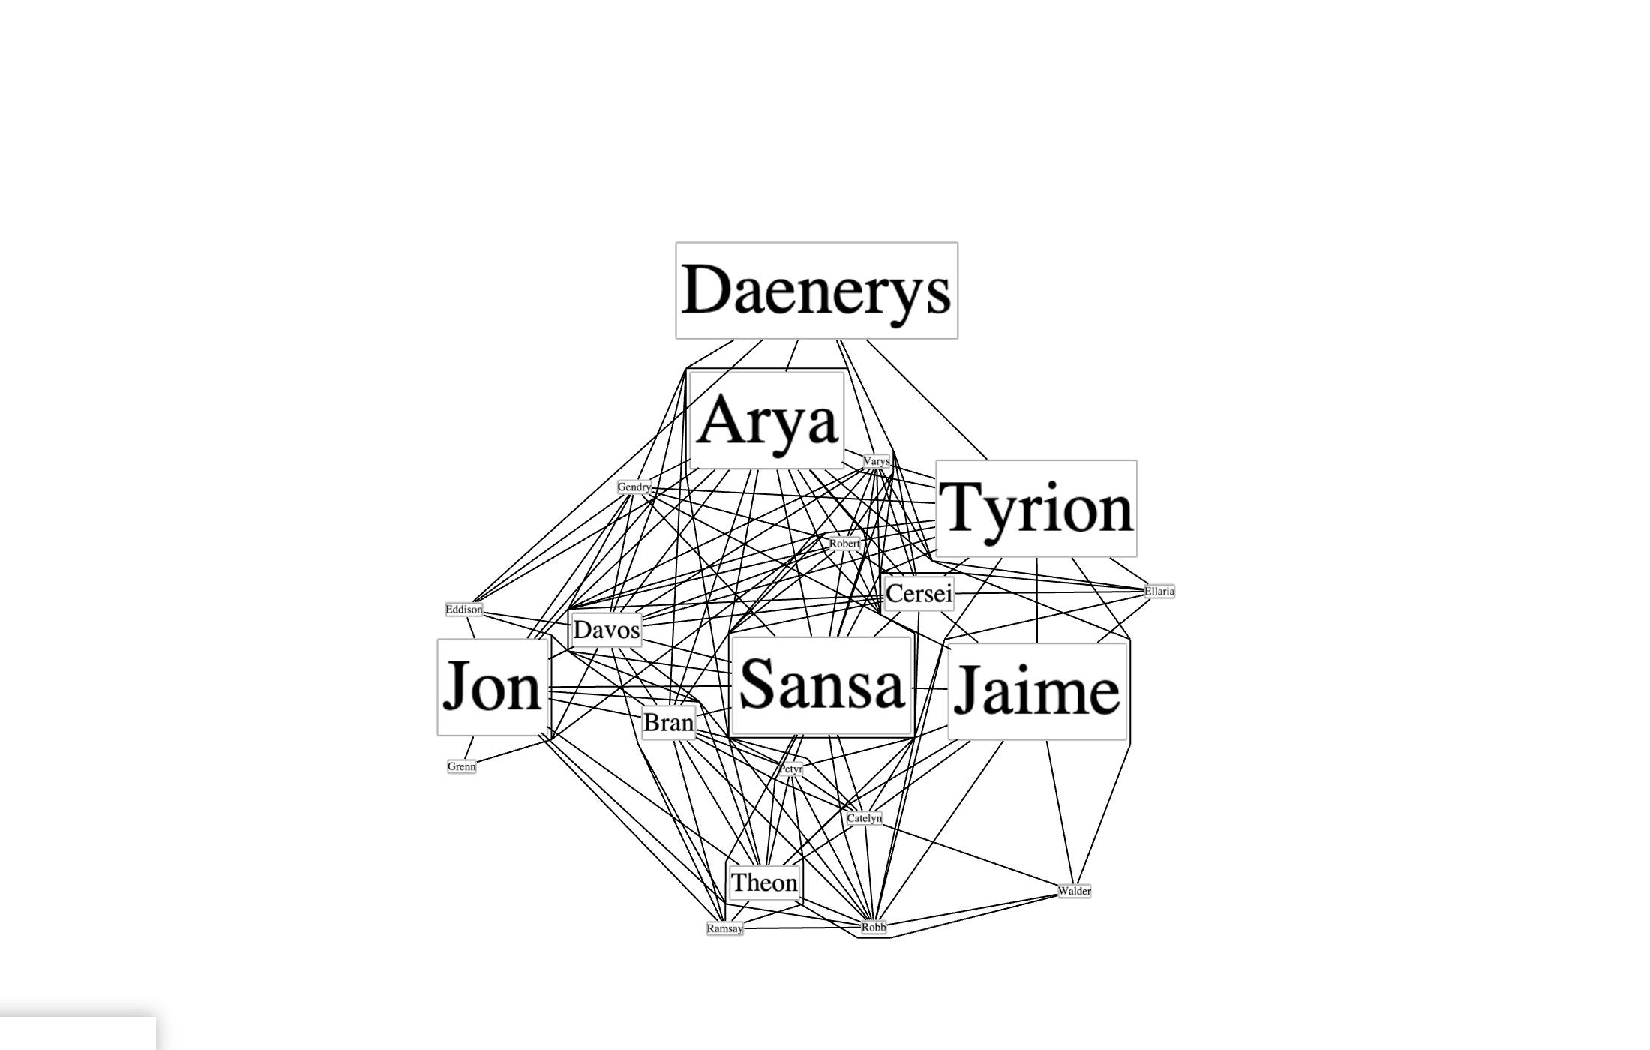
\includegraphics[width=0.49\linewidth]{got_top_coarse.pdf}\hfill
  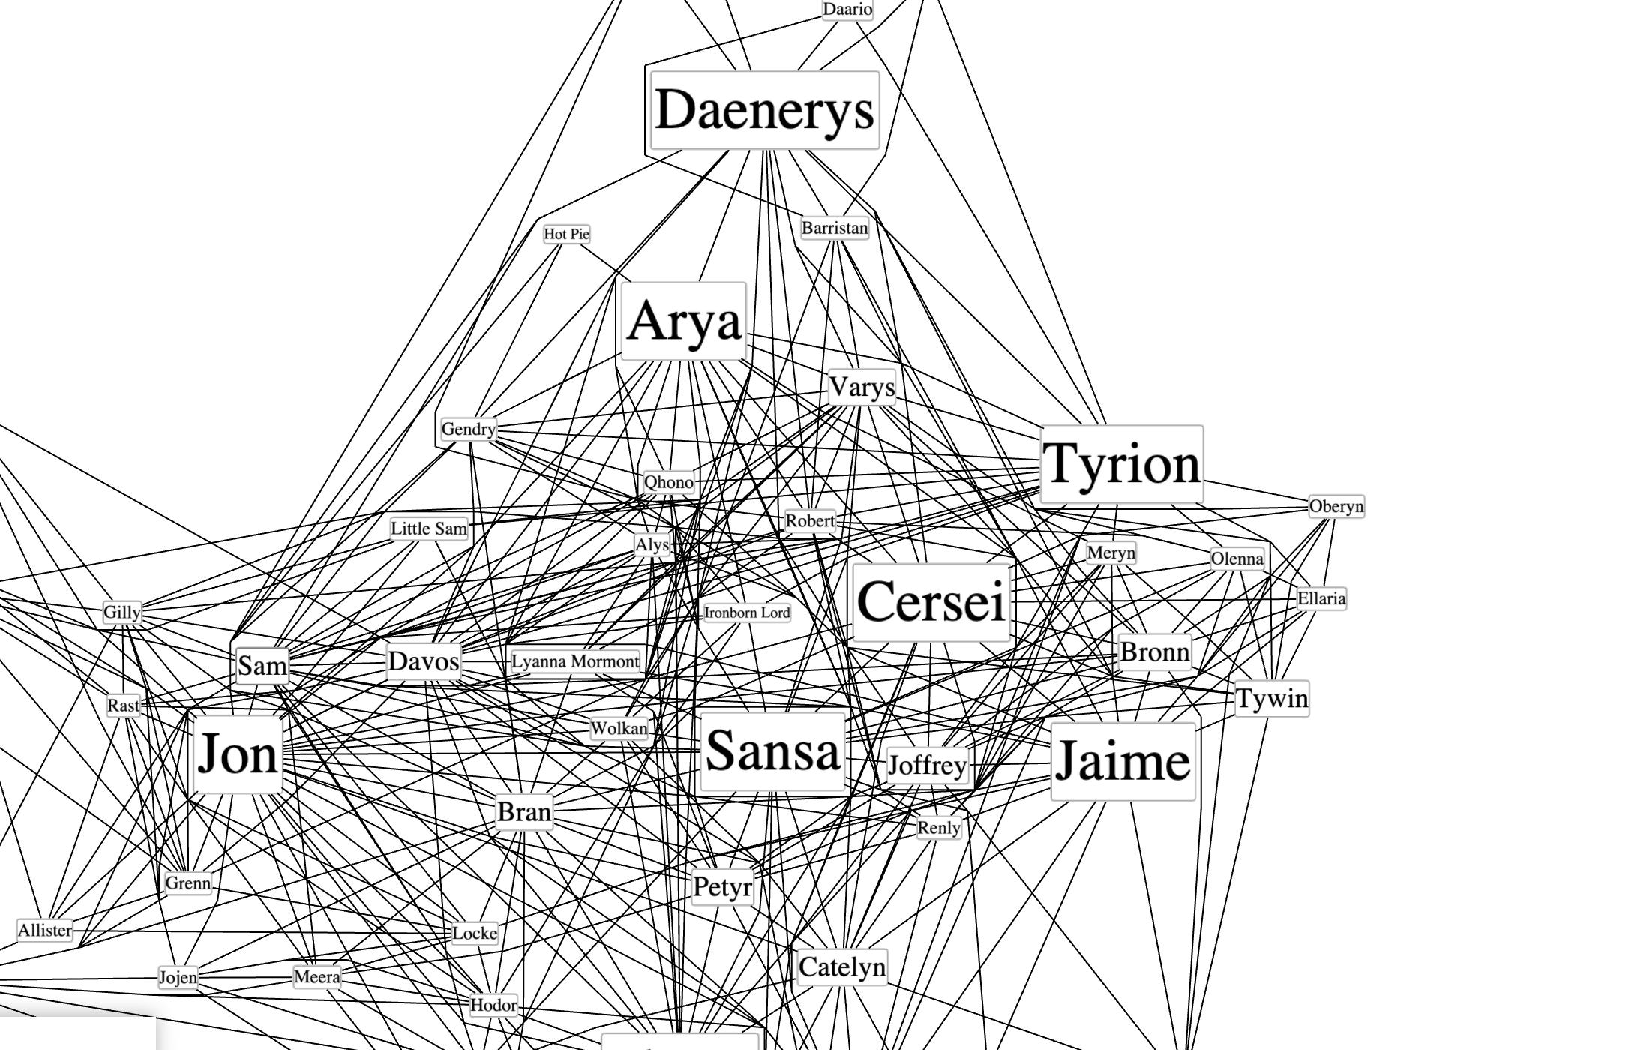
\includegraphics[width=0.49\linewidth]{got_top_fine.pdf}
  \caption{Two adjacent pyramid levels of the Game of Thrones graph
    rendered by the WebGL renderer of \msagljs{} with the sleeve
    router. The coarser level is on the left, the finer one on the
    right; both panels are cropped to the same world window. For each
    level a new graph is assembled from a PageRank-ranked prefix of
    the nodes, and edges are routed against the obstacles introduced
    at that level.}
  \label{fig:tile-pyramid}
}

\abstract{%
We present a new way to visualize a large graph in the style of
online geographic maps. The method builds a \emph{tile pyramid} for
\emph{semantic zoom}: at every zoom level the labels of the
highest-ranked nodes remain readable, just as the names of major
geographical features stay readable on those maps.

The edges are routed by a method we call \emph{sleeve routing}, which
searches the dual graph of a Constrained Delaunay Triangulation to
select a sequence of triangles through the free space, then applies the
funnel algorithm to compute a shortest path inside the selected
sleeve. We apply several heuristics to speed up the routing.

We implemented our approach in the WebGL renderer of
\msagljs{}\ifthenelse{\boolean{gdanonymous}}{ (a placeholder name used
during double-blind review)}{}, an open-source TypeScript library for
graph visualization in web browsers, with the entire pipeline running
client-side, without a dedicated server. Our benchmark suite contains
nine graphs with up to $32{,}768$ nodes and $236{,}978$ edges, and
measures browser-side parsing, layout, routing, and tile-pyramid
construction. The renderer's demo can be seen at
\anondemourl{\anondemowebgl}{https://microsoft.github.io/msagljs/renderer-webgl-sleeve/index.html};
the sources and packages are described under Supplemental Materials.%
}

\keywords{Graph visualization, edge routing, Constrained Delaunay Triangulation, tiling, WebGL.}

%%%%%%%%%%%%%%%%%%%%%%%%%%%%%%%%%%%%%%%%%%%%%%%%%%%%%%%%%%%%%%%%
%%%%%%%%%%%%%%%%%%%%%% START OF THE PAPER %%%%%%%%%%%%%%%%%%%%%%
%%%%%%%%%%%%%%%%%%%%%%%%%%%%%%%%%%%%%%%%%%%%%%%%%%%%%%%%%%%%%%%%

\begin{document}

\firstsection{Introduction}

\maketitle
\label{sec:intro}

Visualizing graphs in web browsers without a dedicated server presents
practical challenges: long-running computations can block the main
thread unless offloaded to workers, browser memory is limited, and users expect
the smooth pan-and-zoom experience familiar from online
maps. \msagljs{}
is an open-source TypeScript library that addresses these challenges
by combining efficient layout algorithms, a novel edge routing method,
and a tiling scheme with semantic zoom.

\msagljs{} is consumed as a set of NPM packages and renders graphs
using WebGL through the deck.gl framework~\cite{deckgl}. It supports
the layered Sugiyama scheme~\cite{sugiyama1981}, Pivot
MDS~\cite{brandes2007eigensolver}, and
IPSep-CoLa~\cite{dwyer2006ipsepcola}, with edges routed around node
obstacles. Throughout this paper our typical example is a social
network laid out by IPSep-CoLa; the methods we describe, however, are
agnostic to the layout algorithm and apply to any node placement in
which the nodes do not overlap. The graph loading pipeline builds a
hierarchy of tiles---analogous to map tiles---so that at any zoom
level only the entities in visible tiles are drawn. The capacity
parameter guides pyramid construction but is not a hard bound on
rendered tile occupancy. Tiles are supplied locally
to the browser through the standard \texttt{TileLayer} of the
\texttt{@deck.gl/geo-layers} package, giving smooth pan and zoom. A live
demo of the WebGL renderer is available
online\footnote{\anondemourl{\anondemowebgl}{https://microsoft.github.io/msagljs/renderer-webgl-sleeve/index.html}}.

This paper makes two main contributions:
\begin{enumerate}
\item A \emph{tiling scheme} for large graph visualization that builds
  a hierarchical tile pyramid, reduces the number of visible entities using
  PageRank-based filtering and edge-clip bundling, and integrates with
  the WebGL renderer for interactive pan and zoom.
\item A \emph{sleeve routing} algorithm that selects triangle
  sequences on the dual graph of a Constrained Delaunay Triangulation
  using per-source batched Dijkstra searches, then applies the
  classical funnel algorithm to find shortest paths within the
  selected sleeves. Sleeve selection is heuristic, not globally
  shortest-path optimal.
\end{enumerate}

%% ═══════════════════════════════════════════════════════════════════
\section{Related Work}
\label{sec:related}

\paragraph{Graph visualization tools.}
Graphviz~\cite{gansner2000graphviz,graphviz} is a long-standing graph
drawing tool supporting multiple layout algorithms, including the
Sugiyama method and Scalable Force-Directed Placement~\cite{sfdp}; it
does not support tiling or WebGL rendering. \ifthenelse{\boolean{gdanonymous}}{MSAGL~\cite{nachmanson2004glee} is a
desktop layout engine that did not have the features described here.}{\msagljs{} builds on the
earlier MSAGL desktop layout engine~\cite{nachmanson2004glee} that did
not have the features described here.} On the web,
Sigma.js~\cite{sigmajs} and Cytoscape.js~\cite{franz2016cytoscape}
provide interactive graph rendering, but rely on straight-line or
generic spline edges without obstacle-avoiding routing and without a
pyramid of precomputed tiles. ReGraph~\cite{regraph} uses WebGL to
render large graphs with straight-line edges and supports interactive
cluster expansion but not tiling. Cosmograph~\cite{cosmograph} uses
GPU-accelerated force-directed layout for million-node graphs with
straight-line edges, without
tiling. GraphMaps~\cite{nachmanson2015graphmaps} introduced the
tile-pyramid and node-ranking scheme\ifthenelse{\boolean{gdanonymous}}{}{ on which we build}, but it runs
only on Windows, ships raster tiles, and reuses one global edge
routing that is merely clipped per tile; \msagljs{} brings the idea to
the browser with vector tiles and per-level sleeve routing. Cornac~\cite{perrot2018cornac} handles huge
graphs with tiles and edge
bundling~\cite{hurter2012graph,holten2009fdeb} but requires a
multi-server backend. Earlier navigation schemes for large graphs
include ASK-GraphView~\cite{abello2006askgraphview}, which organizes
nodes into a hierarchical cluster tree, and topological fisheye
views~\cite{gansner2005topological}, which distort a multilevel
layout~\cite{harel2002multiscale,hu2005efficient} under the focus;
neither targets browser-side tile pyramids or per-level edge
routing. Hierarchical edge bundling~\cite{holten2006hierarchical}
and force-directed bundling~\cite{holten2009fdeb} offer alternative
clutter-reduction strategies; but neither method guarantees that
 bundled edges avoid node obstacles.
\paragraph{Shortest paths and edge routing.}
Our sleeve algorithm walks the dual of a Constrained Delaunay
Triangulation~\cite{shewchuk2002delaunay} and relies on the classical
funnel algorithm for extracting a geodesic from a triangle
strip~\cite{lee1984euclidean,chazelle1982theorem,guibas1987linear,pathOpt}.
The optimal algorithm for Euclidean shortest paths among polygonal
obstacles~\cite{hershberger1999optimal} and the recent
$O(m\log^{2/3} n)$ single-source shortest-path algorithm that breaks
the sorting barrier~\cite{duan2025sorting} are remarkable theoretical
results. We do not implement or benchmark these algorithms; our
engineering choice is to reuse a CDT and conventional graph searches.
Graphviz builds the full visibility graph for edge routing in force-directed layouts, which has $O(n^2)$ edges. For Sugiyama layouts, it uses the funnel algorithm~\cite{dobkin1997implementing} but requires a simple containing polygon. yWorks~\cite{yworks} offers ``Organic edge routing'' based on force-directed simulation. The approach of Dwyer and Nachmanson~\cite{dwyer2010fast} routes on a Yao-graph spanner with local shortcutting. For orthogonal layouts, the libavoid framework of Wybrow, Marriott, and Stuckey performs obstacle-avoiding connector routing with incremental updates~\cite{wybrow2010orthogonal}.

\paragraph{CDT-based pathfinding.}
The closest precedent to our routing pipeline is the CDT-and-funnel
pathfinder of Demyen and Buro~\cite{demyen2006efficient}, originally
designed for game-AI units of nonzero radius. They run admissible A*
search on the CDT dual (with a reduced-graph variant that collapses
corridor chains into single abstract edges) to recover provably
shortest paths. Their search is, however, per-query: the bounds depend
on the start and goal, so it cannot share work across the edges with
the same source as our per-source Dijkstra does. For the graphs we
target, sharing work across queries is attractive. We trade a
global optimality guarantee for batched search; we have not
benchmarked their pathfinder directly, so we make no quantitative
speed comparison with it.


%% ═══════════════════════════════════════════════════════════════════
\section{Tiling}
\label{sec:tiling}
The input to tiling is a laid-out graph together with routed edges.
We use sleeve routing, Section~\ref{sec:sleeve-routing}, both for the
input graph and for the coarser levels; routes at different levels
are computed independently, so continuity across level changes is
not guaranteed. The output is a sequence of $Z{+}1$ levels: level~$Z$
is the finest, and level~$0$ is the coarsest. Each level is a
collection of tiles indexed by integer $(x,y)$ grid coordinates.

A tile is an axis-aligned square together with its \emph{tile data}:
nodes, edge labels, edge arrowheads, and \emph{edge clips}. An edge
clip is a curve confined to the tile square, paired with the
non-empty list of graph edges whose clipped routes have the same
quantized endpoint pair including endpoints inside the tile.
Bundles are intended to capture stretches on which
several routes travel close together inside a common sleeve; we
represent each such stretch as a single clip with an attached edge
list, rather than as one clip per edge.
All tiles at level~$z$ have side length $\ell_z=\ell_0/2^z$,
where $\ell_0$ is the root tile's side length. Each subdivision
produces four congruent square sub-tiles of half the parent's side length.

Pseudocode~\ref{alg:build-pyramid} describes the algorithm building
the tile pyramid.
\begin{algorithm}[t]
\caption{\textsc{BuildTilePyramid}$(G, \mathcal{C}, \mathcal{M}_{\max})$}
\label{alg:build-pyramid}
\begin{algorithmic}[1]
\State $T_0 \gets$ single square tile of side $\ell_0=2^{\lceil \log_2 \max(w,h)\rceil}$ centered on $G$'s bounding box of width $w$ and height $h$, holding all of $G$
\State $(\bar w,\bar h) \gets$ mean original node width and height
\State $\mathit{levels} \gets [\,T_0\,]$;\quad $z \gets 0$;\quad $\mathit{used} \gets |T_0|$ \Comment{$|T|$ = element count of tile $T$}
\While{some tile in $\mathit{levels}[z]$ exceeds $\mathcal{C}$ elements}
  \State $\mathit{next} \gets$ empty $2^{z+1}{\times}2^{z+1}$ tile grid
  \ForAll{tiles $T \in \mathit{levels}[z]$} \Comment{per-tile inner loop}
    \State split $T$ into four congruent square sub-tiles of $\mathit{next}$ \label{algln:split}\Comment{Section~\ref{sec:tile-build}}
    \State $\mathit{used} \mathrel{+}=$ number of new elements added to $\mathit{next}$
    \If{$200 \cdot \mathit{used} > \mathcal{M}_{\max}$} \Comment{memory budget; checked mid-split}
      \State \textbf{discard} $\mathit{next}$ and \textbf{break} pyramid growth
    \EndIf
  \EndFor
  \State $\mathit{levels}[z{+}1] \gets \mathit{next}$;\quad $z \gets z + 1$
  \If{$\ell_z \leq 10\min(\bar w,\bar h)$}
    \State \textbf{break} \Comment{retain this completed level}
  \EndIf
\EndWhile
\State $Z \gets z$;\quad $V_Z \gets V(G)$;\quad $s_v^{(Z)} \gets 1$ for all $v\in V_Z$
\State $V_{\mathrm{PR}} \gets$ nodes of $G$ sorted by descending PageRank
\For{$z = Z-1$ \textbf{down to} $0$}
  \State $P_z \gets$ first $\lceil |V|/2^{Z-z}\rceil$ nodes of $V_{\mathrm{PR}}$, restricted to $V_{z+1}$
  \State $(V_z, \{s_v^{(z)}\}) \gets$ \textsc{SelectTopKWithAdaptiveScale}$(P_z)$ \Comment{Section~\ref{sec:filter}}
  \State $E_z \gets \{uv\in E(G): u,v\in V_z\}$
  \State build a CDT from the inflated polylines of $V_z$ at scales $\{s_v^{(z)}\}$
  \State route every edge $e\in E_z$ on this CDT
  \State rebuild the tiles of $\mathit{levels}[z]$ \label{algln:rebuild}\Comment{Section~\ref{sec:tile-build}}
\EndFor
\State \Return $\mathit{levels}$
\end{algorithmic}
\end{algorithm}


\begin{figure}[!tb]
  \centering
  \resizebox{0.95\linewidth}{!}{%
  \begin{tikzpicture}[
      x={(1.0cm,0cm)},
      y={(0.40cm,0.60cm)},
      z={(0cm,1.0cm)},
      line cap=round,
    ]
    \def\W{2.0}      %% slab half-width in cm; slab is square, span (-W,-W)..(W,W).
    \def\dh{1.4}     %% vertical spacing between slabs
    %% Pan center for the user's viewport on each slab (in slab cm).
    %% At z=3, with this center the worked-example viewport intersects
    %% exactly the 3x2 = 6 tiles required by the body text.
    \def\cx{-0.25} \def\cy{0}
    %% Screenshot is 1226x950 px. At view zoom v = z-1 (the integer zoom
    %% that snaps to level z when v_0=-1), the viewport in world units is
    %% (1226/2^v) x (950/2^v). With the slab's full width 2W = 4 cm
    %% representing the W=1024 wu world, half-extents in cm are
    %% hx = 1226/(512*2^v) and hy = 950/(512*2^v).
    \pgfmathsetmacro{\iwfull}{2*\W}
    %% Painter's order: bottom (z=4) up to top (z=0).
    \foreach \zlev/\h in {%
        4/0,%
        3/1,%
        2/2,%
        1/3,%
        0/4%
      } {
      \pgfmathtruncatemacro{\nn}{int(2^\zlev)}
      \pgfmathsetmacro{\step}{2*\W/\nn}
      \pgfmathsetmacro{\twov}{pow(2,\zlev-1)}
      \pgfmathsetmacro{\hx}{1226/(512*\twov)}
      \pgfmathsetmacro{\hy}{950/(512*\twov)}
      %% Slab outline with a faint fill so the empty area is visibly empty.
      \filldraw[fill=blue!4, draw=blue!55, line width=0.5pt]
        (-\W,-\W,\h*\dh) -- (\W,-\W,\h*\dh) -- (\W,\W,\h*\dh) -- (-\W,\W,\h*\dh) -- cycle;
      %% Place the LOD screenshot. Always render the screenshot at its
      %% actual viewport size in slab cm, centered at the pan point. For
      %% z<2 this rectangle exceeds the slab, but the slab clip leaves
      %% only the world-content portion visible, which then exactly
      %% fills the slab. For z>=2 the rectangle fits inside the slab,
      %% leaving the rest visibly empty.
      \pgfmathsetmacro{\iw}{2*\hx}
      \pgfmathsetmacro{\ih}{2*\hy}
      \pgfmathsetmacro{\vxa}{\cx-\hx}
      \pgfmathsetmacro{\vya}{\cy-\hy}
      \begin{scope}
        \clip (-\W,-\W,\h*\dh) -- (\W,-\W,\h*\dh) -- (\W,\W,\h*\dh) -- (-\W,\W,\h*\dh) -- cycle;
        \begin{scope}[shift={(\vxa,\vya,\h*\dh)}]
          \pgflowlevelsynccm
          \pgftransformcm{1}{0}{0.40}{0.60}{\pgfpointorigin}
          \pgftext[base,left]{%
            %% arXiv's static scanner cannot expand \foreach loop variables,
            %% so each filename is written out literally here.
            \ifcase\zlev
              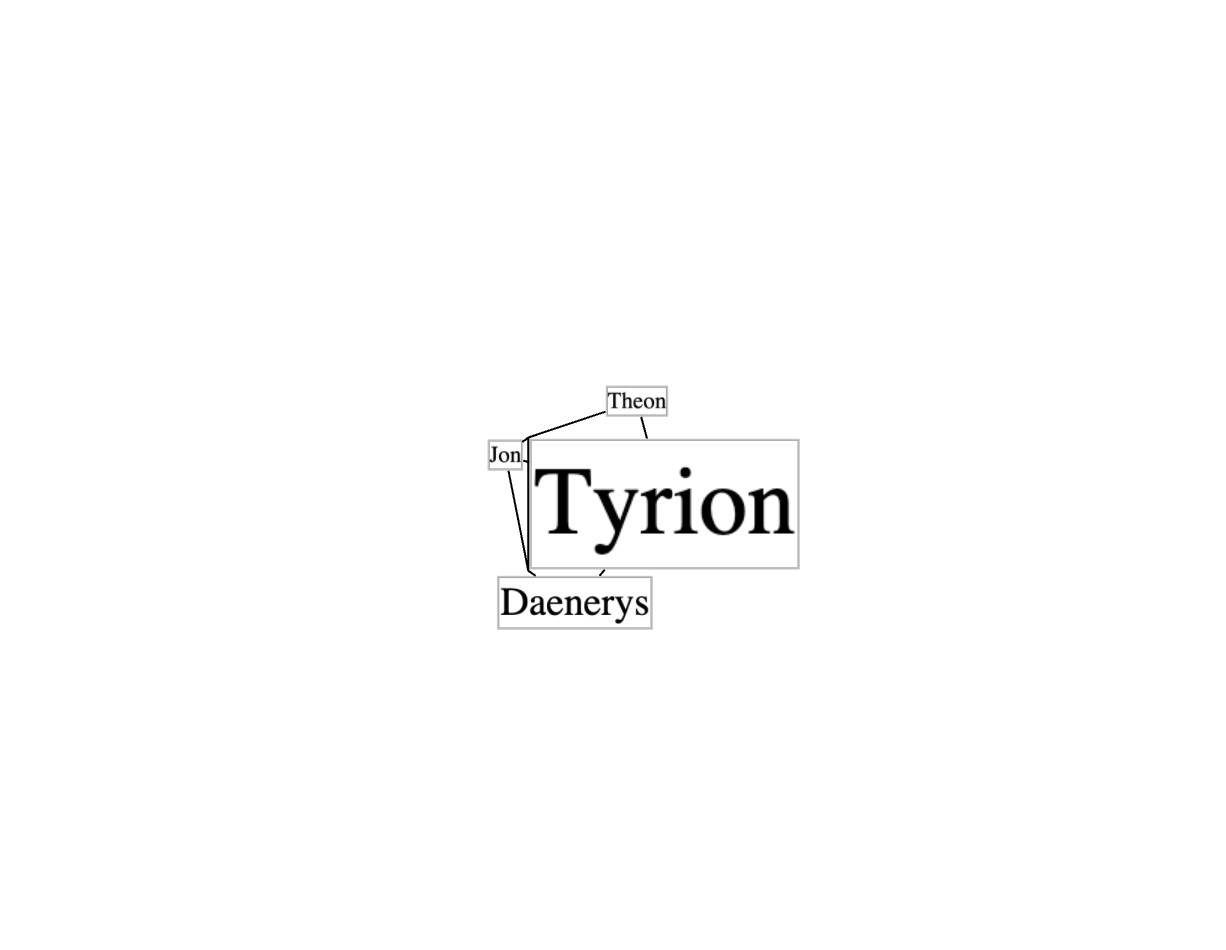
\includegraphics[width=\iw cm, height=\ih cm]{got_view_z0.png}\or
              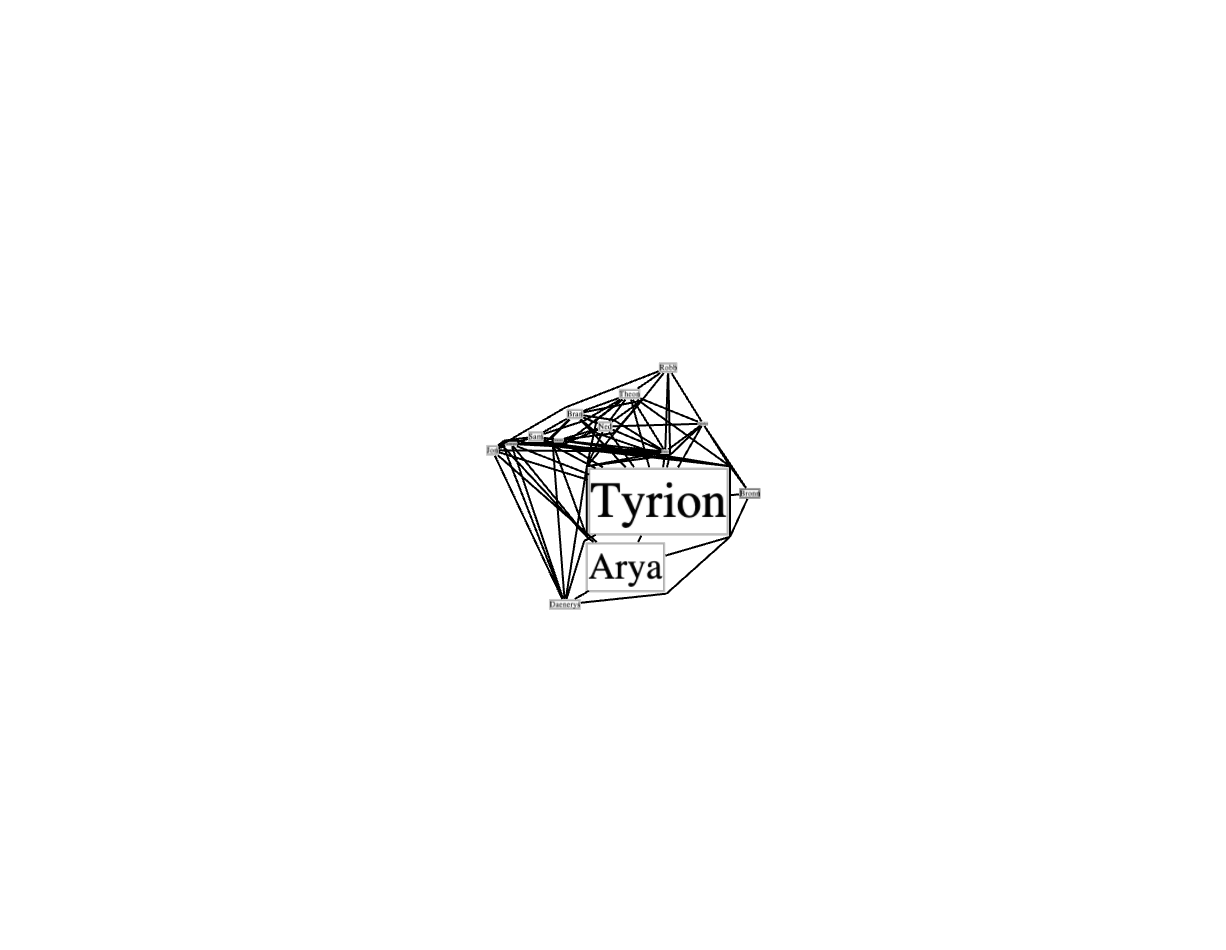
\includegraphics[width=\iw cm, height=\ih cm]{got_view_z1.png}\or
              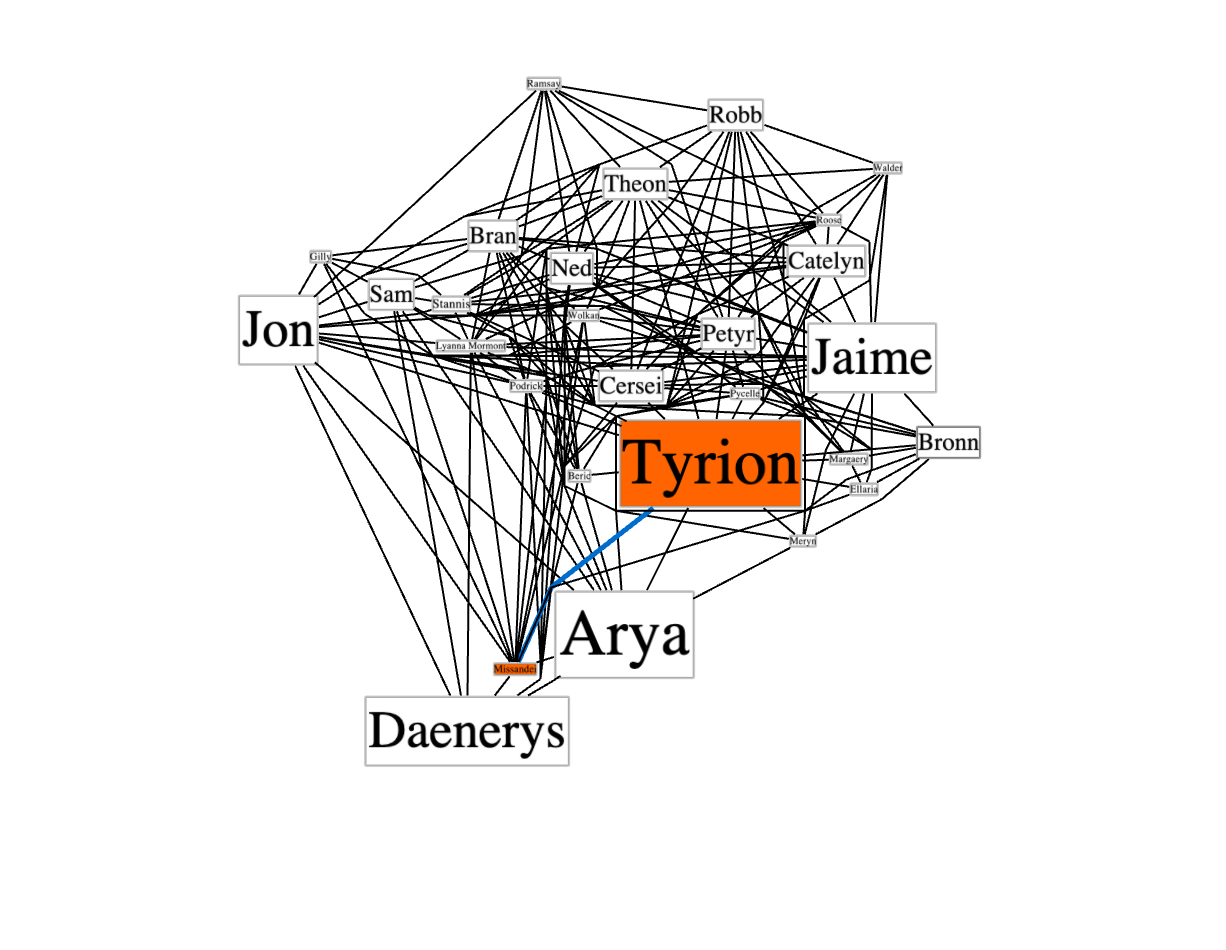
\includegraphics[width=\iw cm, height=\ih cm]{got_view_z2.png}\or
              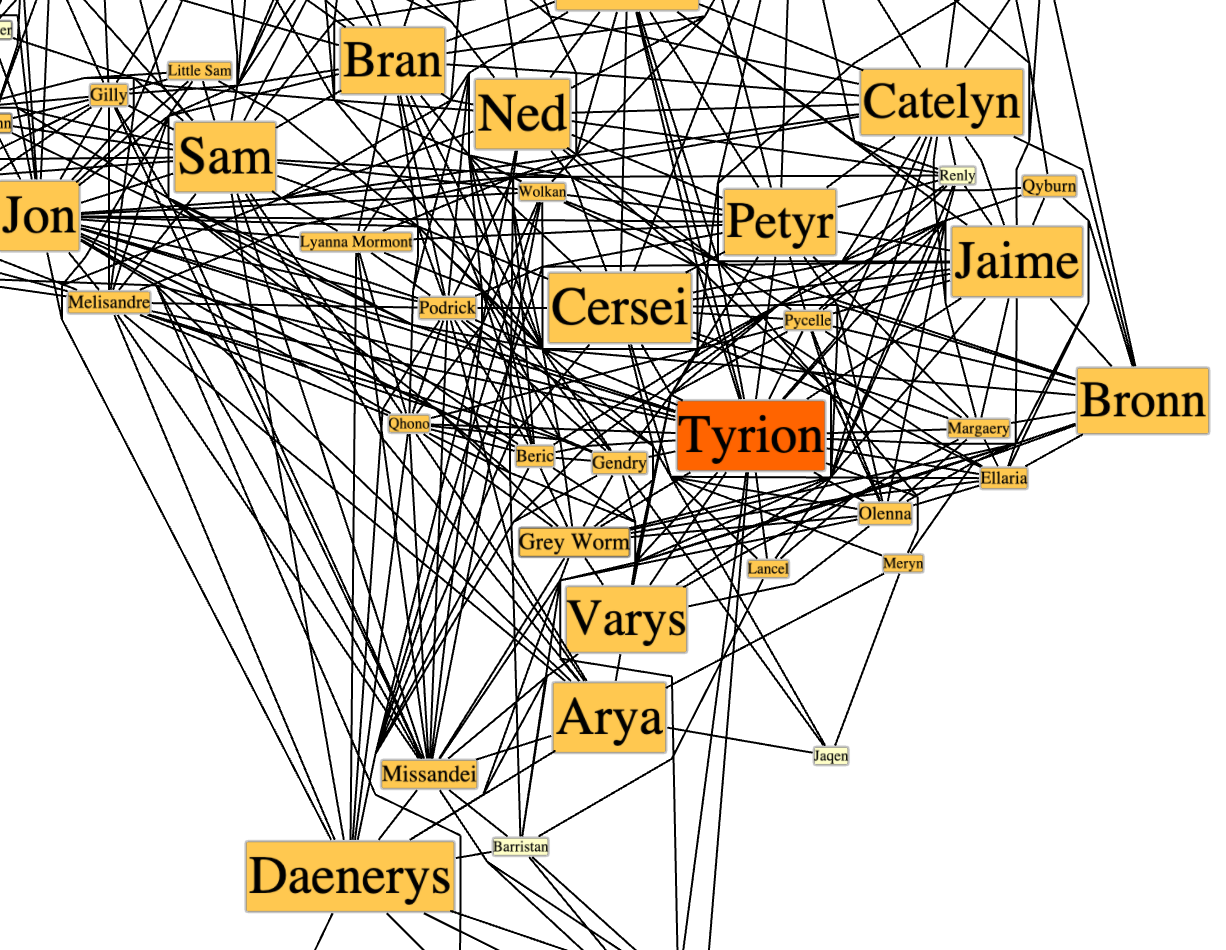
\includegraphics[width=\iw cm, height=\ih cm]{got_view_z3.png}\or
              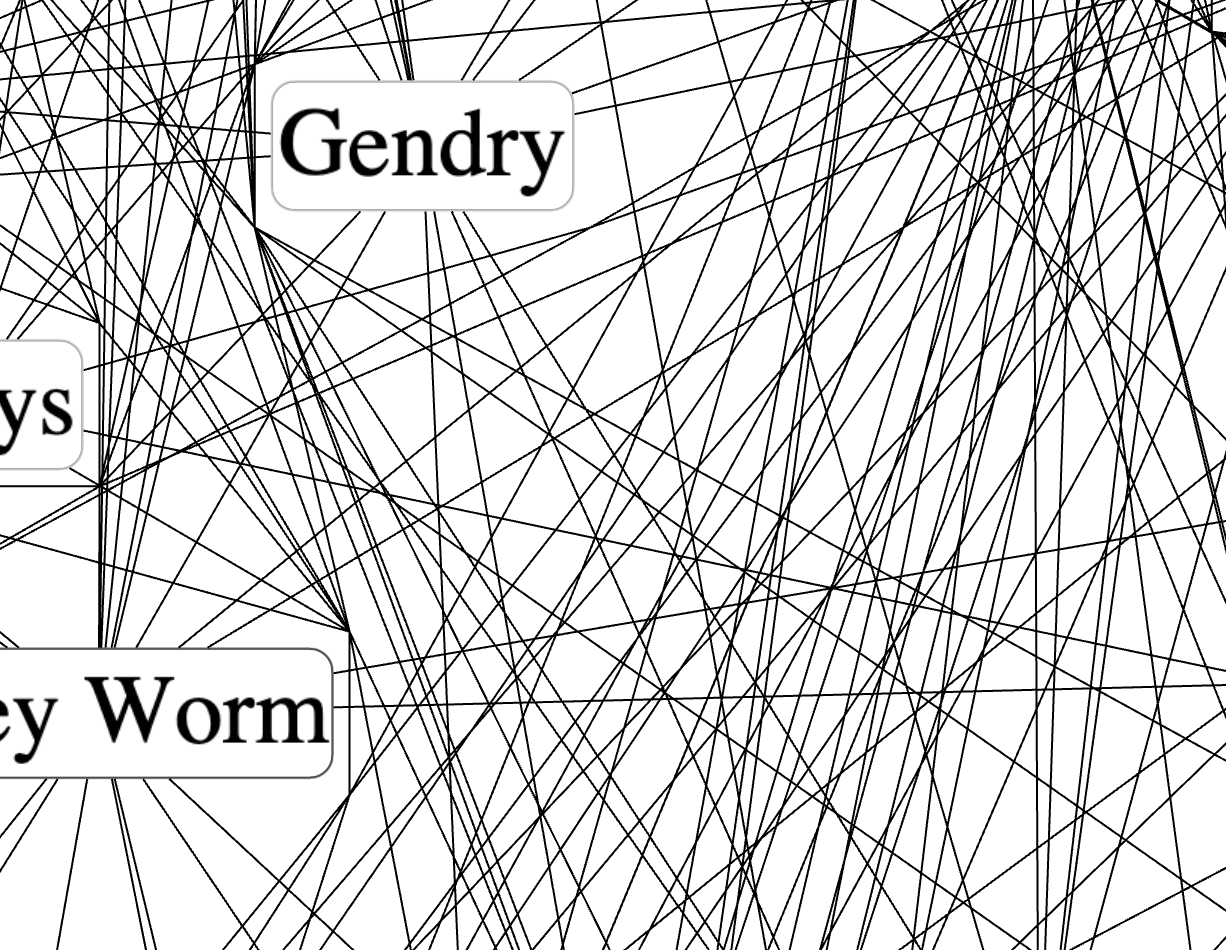
\includegraphics[width=\iw cm, height=\ih cm]{got_view_z4.png}%
            \fi}
        \end{scope}
      \end{scope}
      %% Faint tile grid: 2^z x 2^z square cells.
      \ifnum\nn>1
        \foreach \i in {1,...,\numexpr\nn-1\relax} {
          \pgfmathsetmacro{\u}{-\W + \i*\step}
          \draw[blue!50, line width=0.25pt] (\u,-\W,\h*\dh) -- (\u,\W,\h*\dh);
          \draw[blue!50, line width=0.25pt] (-\W,\u,\h*\dh) -- (\W,\u,\h*\dh);
        }
      \fi
      %% Worked example at z=3: outline the 3 x 2 = 6 tiles fetched at v=2.
      \ifnum\zlev=3
        \pgfmathsetmacro{\vxa}{\cx-\hx} \pgfmathsetmacro{\vxb}{\cx+\hx}
        \pgfmathsetmacro{\vya}{\cy-\hy} \pgfmathsetmacro{\vyb}{\cy+\hy}
        \pgfmathtruncatemacro{\ia}{floor((\vxa+\W)/\step)}
        \pgfmathtruncatemacro{\ib}{floor((\vxb+\W)/\step)}
        \pgfmathtruncatemacro{\ja}{floor((\vya+\W)/\step)}
        \pgfmathtruncatemacro{\jb}{floor((\vyb+\W)/\step)}
        \foreach \i in {\ia,...,\ib} {
          \foreach \j in {\ja,...,\jb} {
            \pgfmathsetmacro{\xa}{-\W + \i*\step}
            \pgfmathsetmacro{\xb}{-\W + (\i+1)*\step}
            \pgfmathsetmacro{\ya}{-\W + \j*\step}
            \pgfmathsetmacro{\yb}{-\W + (\j+1)*\step}
            \draw[orange!75!black, line width=0.7pt]
              (\xa,\ya,\h*\dh) -- (\xb,\ya,\h*\dh) -- (\xb,\yb,\h*\dh) -- (\xa,\yb,\h*\dh) -- cycle;
          }
        }
      \fi
      %% Per-slab label on the front-left, where no slab above can occlude it.
      \node[anchor=east, font=\scriptsize] at (-\W-0.05, -\W, \h*\dh)
        {$z{=}\zlev$\,(\nn${\times}$\nn)};
    }
  \end{tikzpicture}}
  \caption{Tile grids and viewports at five pyramid levels. Each
    screenshot uses its level's display sizes and zoom; the blue grid
    shows the full world extent. The orange outlines mark the six
    tiles intersected by the viewport at level~3.}
  \label{fig:tile-pyramid-3d}
\end{figure}

\paragraph{How the index of the finest level, $Z$, is chosen.}
For this task we build the pyramid without element filtering: every
level contains all graph entities. Starting from the root tile, we
keep adding levels and splitting tiles until a stopping condition is
met; the index of the finest level built this way is $Z$. The finest
level is kept as is, while the tiles of levels~$0, \ldots, Z-1$ are
later rebuilt as described below.

Let $w_v$ and $h_v$ be the width and height of node~$v$'s
axis-aligned bounding box in the original layout, before padding or
level-dependent scaling. For the non-cluster nodes $V$, define
\[
  \bar w=\frac{1}{|V|}\sum_{v\in V}w_v,\qquad
  \bar h=\frac{1}{|V|}\sum_{v\in V}h_v.
\]
We denote by $\ell_k$ the length of a tile side on level $k$.

We start from $Z=0$; if the root tile already meets the capacity
condition, no subdivision is needed. Otherwise we grow the pyramid
one level at a time and stop as soon as any of three conditions is met:
\begin{enumerate}
\item every tile at the new level contains at most $\mathcal{C}$
elements, with default $\mathcal{C}=500$;
\item the completed new level~$z$ satisfies
  $\ell_z\leq 10\min(\bar w,\bar h)$.
  Equivalently, the side length is at most ten times both the mean
  node width and the mean node height; equality triggers the stop.
  This level is retained as the finest level, $Z=z$;
\item the total of stored tile elements summed over all levels, multiplied by
$200$~bytes per element, exceeds the memory budget $\mathcal{M}_{\max}$,
with default $4$~GiB ($2^{32}$ bytes); the partial level is then discarded and $Z$ is
set to the previous finest level.
\end{enumerate}
The third condition is checked incrementally inside the level-build
loop. This is a storage estimate, not a bound on the browser's actual
heap: it does not account for all object overhead, edge-membership
lists, routing workspace, or GPU buffers, and is not rechecked during
the subsequent per-level rebuilding. In our experiments, on every
benchmark graph in Table~\ref{tab:max-per-tile} the first condition
fires; the second and third are defensive guards that bound $Z$ on
hypothetical inputs with extremely densely positioned entities.
\paragraph{Three phases.} Once $Z$ is fixed,
each coarser level $z=Z{-}1, Z{-}2, \dots, 0$ is built in three
phases:
\begin{enumerate}
\item choose some of the nodes of level~$z+1$ as the nodes of
  level~$z$, guided by PageRank, and possibly enlarge them,
  Section~\ref{sec:filter};
\item reroute the edges of $G_z$ around the resulting obstacles,
  Section~\ref{sec:sleeve-routing};
\item recompute the per-tile edge clips on level $z$,
  Section~\ref{sec:tile-build}.
\end{enumerate}
Figure~\ref{fig:tile-pyramid} shows two adjacent pyramid levels built
by this procedure; Algorithm~\ref{alg:build-pyramid} summarizes the
whole pipeline.

\subsection{PageRank-Guided Level Construction}
\label{sec:filter}
We compute PageRank~\cite{page1999pagerank} on $G$ once and sort the
nodes by descending rank; from now on we think of $V$ as this sorted
array.

The levels are built from fine to coarse. We add nodes to level $z$
by walking its \emph{prefix}: the first $\lceil|V|/2^{Z-z}\rceil$
nodes of $V$, skipping the nodes that were not accepted at
level~$z+1$. We do not change the node
positions inherited from the finest level, but we try to increase the
scale of the nodes. The top-ranked node is scaled by $2^{Z-z}$. We keep the node
scales non-increasing, but as large as possible, while making sure
that each next node does not overlap the previously selected nodes of
the level, with the routing padding included in the overlap test. Each
accepted scale lies between $1$ and the preceding accepted scale. If
even at scale~$1$ the candidate's padded bounding box would overlap an
already-accepted node's padded scaled box, the candidate is dropped.

Dropping a relatively high-ranked candidate at a coarse level is a
deliberate compromise: we trade the inclusion of that candidate at
this level for the invariant that the rendered nodes at every level
remain pairwise disjoint. The cost is small in practice. Consider
Cersei's node in the \emph{Game of Thrones} graph: it is dropped from
the coarsest level because a higher-ranked node, Tyrion, has covered
the available region. The user still sees that part of the graph as
occupied, and Cersei's individual node appears on the next, finer
level, where its box fits. All nodes are present at the finest level.

Let $V_z$ be the nodes accepted at level $z$. The level graph is
$G_z=(V_z,E_z)$, where $E_z=\{uv\in E(G): u,v\in V_z\}$: the edges of
the level are those connecting two level nodes. Because the
candidates for level $z$ are drawn from the nodes accepted at
level~$z+1$, the accepted sets are nested: $V_z\subseteq V_{z+1}$.
A node visible at some level therefore stays visible at every finer
level. The restriction also speeds up the filter: a node rejected at
some level is not reconsidered at the coarser ones.

\paragraph{Spatial-hash overlap test.}
A naive overlap test against every previously accepted node takes
time quadratic in the number of nodes to position and would
dominate the cost of the filter. We view the plane as
subdivided into a conceptual uniform grid of square cells of
side~$c$: the cell of a point $(x,y)$ is the integer pair
$(\lfloor x/c\rfloor, \lfloor y/c\rfloor)$, and the grid itself is
never built. Instead, every accepted box is stored in a hash table
keyed by the cell of its center~\cite{teschner2003optimized}
(Figure~\ref{fig:spatial-hash}). Only non-empty cells occupy memory,
so the storage is proportional to the number of accepted boxes,
independent of the layout extent. The cell side is fixed per level as
$c = 2^{Z-z} d_{\max} + 2m$, where $d_{\max}$ is the largest among
the widths~$w_v$ and heights~$h_v$ of the level's candidates~$v$,
and $m$ is the margin by which each box side is padded in the
overlap test. Since $2^{Z-z}$ is the level's maximum
scale, no tested box, accepted or candidate, is wider or taller than
one cell. Each
box then extends at most half a cell side from its center, so the
centers of two overlapping boxes lie less than one cell side apart on
each axis, and their cells are identical or adjacent. A box
registered two or more cells away cannot intersect the candidate. Testing a candidate therefore takes at most nine
hash-table queries---one for its own cell and one for each of the
eight neighbors---each followed by an overlap check against the
boxes stored in the retrieved cell; the test stops as soon as the
candidate is rejected.

\begin{figure}[tb]
  \centering
  \resizebox{0.9\linewidth}{!}{%
  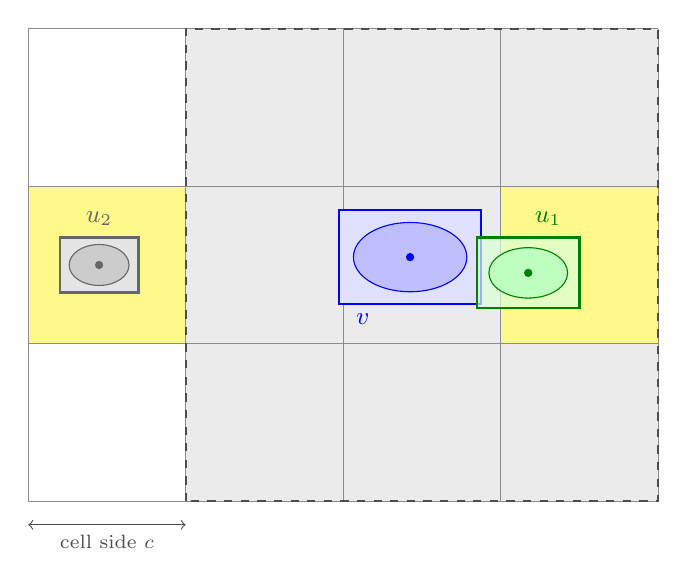
\begin{tikzpicture}[x=1cm,y=1cm]
    \def\c{2.0}
    % 3x3 neighborhood of the candidate's cell
    \fill[black!8] (\c,0) rectangle (4*\c,3*\c);
    % occupied cells: cells holding the center of a stored box
    \fill[yellow!45] (3*\c,\c) rectangle (4*\c,2*\c);
    \fill[yellow!45] (0,\c) rectangle (\c,2*\c);
    \draw[step=\c, black!45, thin] (0,0) grid (4*\c,3*\c);
    \draw[black!70, dashed, thick] (\c,0) rectangle (4*\c,3*\c);
    \draw[<->, black!70] (0,-0.3) -- (\c,-0.3)
      node[midway, below, font=\scriptsize] {cell side $c$};
    % candidate: padded box at the level's maximum scale (one full
    % cell in extent) with the node ellipse inside
    \draw[blue, thick, fill=blue!12] (3.95,2.5) rectangle (5.75,3.7);
    \draw[blue, fill=blue!25] (4.85,3.1) ellipse [x radius=0.72, y radius=0.44];
    \fill[blue] (4.85,3.1) circle (1.5pt);
    \node[blue, below, font=\small] at (4.25,2.5) {$v$};
    % smaller accepted box in an adjacent cell; the padded boxes overlap
    \draw[green!50!black, thick, fill=green!15, fill opacity=0.7]
      (5.7,2.45) rectangle (7.0,3.35);
    \draw[green!50!black, fill=green!25] (6.35,2.9) ellipse [x radius=0.5, y radius=0.32];
    \fill[green!50!black] (6.35,2.9) circle (1.5pt);
    \node[green!50!black, above, font=\small] at (6.6,3.38) {$u_1$};
    % small accepted box stored two cells away: cannot intersect the candidate
    \draw[black!60, thick, fill=black!10] (0.4,2.65) rectangle (1.4,3.35);
    \draw[black!60, fill=black!20] (0.9,3.0) ellipse [x radius=0.38, y radius=0.26];
    \fill[black!60] (0.9,3.0) circle (1.5pt);
    \node[black!60, above, font=\small] at (0.9,3.38) {$u_2$};
  \end{tikzpicture}}
  \caption{The spatial hash of the overlap filter. Nodes are drawn as
    ellipses; the filter tests their padded boxes (rectangles), each
    stored under the cell containing its center (dots). Cells that
    hold a stored box are tinted yellow. The cell side~$c$ equals the
    full extent of the largest box the filter can test, so no tested
    box is wider or taller than one cell; the candidate~$v$ is drawn
    at this extreme, while accepted boxes are typically smaller. If
    two boxes overlap, as the boxes of $v$ and~$u_1$ do, their
    centers lie less than $c$ apart on each axis, so their cells are
    identical or adjacent. Hence $v$ is tested only against the boxes
    stored in the shaded $3{\times}3$ neighborhood of its center
    cell; a box stored outside it, such as $u_2$'s, cannot
    intersect~$v$'s.}
  \label{fig:spatial-hash}
\end{figure}

The hash brings little benefit at the coarsest levels, where the
prefix is short and even a naive scan over the few accepted boxes is
cheap; it pays off at finer levels, where the prefix grows
geometrically. The number of cells examined per candidate is
constant, but their occupancy is not bounded; a query costs time
proportional to the number of boxes in those cells, and the filter
can still take quadratic time in the prefix length in the worst case.
The spatial hash is therefore an acceleration heuristic rather than
a constant-time overlap guarantee.


\subsection{Splitting Edges between Tiles}
\label{sec:tile-build}
We describe edge routing later in Section~\ref{sec:sleeve-routing}, but
for the purpose of this paragraph it is enough to know that each curve
is a polyline.

The edge-clip generation works as follows. Consider a tile and an edge
clip contained in the tile. Let the \emph{midlines} of a tile be the horizontal and
vertical segments through its center; they split the tile into four
congruent square sub-tiles. Cutting the curve with the midlines yields a set of
sub-clips, each contained in one sub-tile. For isolated boundary
contacts, splitting at tangencies as well as crossings ensures that
each sub-clip meets the boundary only at its endpoints. Segments
lying along a midline can be assigned to either incident sub-tile
using a consistent tie-breaking rule. Every split reuses the parent
clip's boundary crossings, and only the curve-vs-midline
intersections need to be computed; no full curve-vs-square clipping
is required. Figure~\ref{fig:clip} illustrates one such split.

\begin{figure}[!tb]
  \centering
  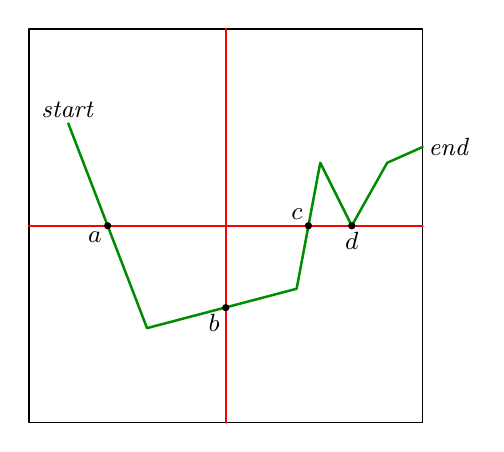
\begin{tikzpicture}[
      line cap=round,
      line join=round,
      every node/.style={font=\small, inner sep=2pt},
    ]
    %% Tile outline.
    \draw[black, line width=0.6pt] (0,0) rectangle (5,5);
    %% Red midlines split the tile into four sub-tiles.
    \draw[red, line width=0.9pt] (0,2.5) -- (5,2.5);
    \draw[red, line width=0.9pt] (2.5,0) -- (2.5,5);
    %% Polyline edge clip from start to end. After the crossing at c
    %% the polyline stays in the UR sub-tile and merely touches the
    %% horizontal midline at d (no crossing). The polyline is
    %% x-monotone, so it does not self-intersect.
    \draw[green!55!black, line width=0.9pt]
         (0.50,3.80)
      -- (1.50,1.20)
      -- (3.40,1.70)
      -- (3.70,3.30)
      -- (4.10,2.50)
      -- (4.55,3.30)
      -- (5.00,3.50);
    %% Dots at the four midline contacts (a, b, c are crossings; d is
    %% a touching point and is itself a polyline vertex).
    \foreach \p in {%
        (1.00,2.50),(2.50,1.46),(3.55,2.50),(4.10,2.50)}
      \filldraw[black] \p circle (1.1pt);
    %% Labels.
    \node[anchor=south]      at (0.50,3.80) {\emph{start}};
    \node[anchor=north east] at (1.00,2.50) {$a$};
    \node[anchor=north east] at (2.50,1.46) {$b$};
    \node[anchor=south east] at (3.55,2.50) {$c$};
    \node[anchor=north]      at (4.10,2.50) {$d$};
    \node[anchor=west]       at (5.00,3.50) {\emph{end}};
  \end{tikzpicture}
  \caption{An edge clip, drawn as a polyline, from \emph{start} to
    \emph{end} inside a tile. The two red midlines split the tile
    into four congruent square sub-tiles and meet the polyline at the four
    points $a$, $b$, $c$, $d$; at $d$ the polyline touches the
    horizontal midline without crossing it. Cutting the polyline at
    these points yields five sub-clips $[\mathit{start},a]$,
    $[a,b]$, $[b,c]$, $[c,d]$, $[d,\mathit{end}]$, each contained in
    one sub-tile and meeting that sub-tile's boundary only at its
    endpoints.}
  \label{fig:clip}
\end{figure}

When we grow the pyramid in line~\ref{algln:split} of
Algorithm~\ref{alg:build-pyramid}, each edge clip is already
contained in its parent tile, so subdivision starts from that
parent's square. When we prepare the tiles for rendering in
line~\ref{algln:rebuild} of Algorithm~\ref{alg:build-pyramid}, we
have the rerouted graph $G_z$, so for each edge of $G_z$ we start
the subdivision from the root tile's square.

\paragraph{Bundling edge clips.}
To reduce the number of elements rendered in a tile, all clips within
a tile that share the same unordered pair of quantized endpoints are
bundled into a single clip whose attached edge list accumulates every
contributing edge. Each endpoint coordinate is rounded to the nearest
multiple of $10^{-6}$ world units. The bundled geometry is taken from the first such
clip encountered during splitting, and the choice is consistent within
each level. This endpoint-based test does not bound the deviation
between the interiors of the original curves and their representative.
Table~\ref{tab:max-per-tile} reports the resulting maximum
number of elements rendered in a single tile across the entire pyramid
for a range of graphs.

% Generated from runs of modules/core/test/layout/maxPerTile.spec.ts
% (capacity C=500, no explicit Z cap; natural stops only).
\begin{table}[t]
\caption{Maximum number of elements rendered in a single tile across
  the whole pyramid for several graphs (capacity $\mathcal{C}=500$;
  $Z$ chosen by the natural stops of Section~\ref{sec:tiling}). The
  capacity~$\mathcal{C}$ only guides the choice of~$Z$; we have no
  tight analytical bound on the actual rendered per-tile element
  count, which is therefore reported empirically. ``At level''
  is the level on which the maximum tile was found. In the worst
  cases, \texttt{ca-HepPh} and \texttt{ca-CondMat}, the densest tile
  holds approximately 5.8$\times$ the nominal capacity~$\mathcal{C}$.}
\label{tab:max-per-tile}
\centering
\scriptsize
\setlength{\tabcolsep}{3.5pt}
\begin{tabular}{lrrrrr}
\toprule
Graph & $|V|$ & $|E|$ & Levels & Max/tile & At level \\
\midrule
gameofthrones      &     407 &   2\,639 & 5 &     324 & 4 \\
composers          &  3\,405 &  13\,832 & 8 &     696 & 3 \\
ca-GrQc            &  5\,242 &  28\,968 & 8 &     304 & 4 \\
ca-HepTh           &  9\,877 &  51\,946 & 8 &  1\,839 & 3 \\
facebook\_combined &  4\,039 &  88\,234 & 9 &     961 & 5 \\
ca-HepPh           & 12\,008 & 236\,978 & 9 &  2\,916 & 3 \\
ca-CondMat         & 23\,133 & 186\,878 & 8 &  2\,920 & 3 \\
deezer\_europe     & 28\,281 &  92\,752 & 8 &  2\,395 & 3 \\
delaunay\_n15      & 32\,768 &  98\,274 & 8 &     283 & 7 \\
\bottomrule
\end{tabular}
\end{table}

%% ═══════════════════════════════════════════════════════════════════
\section{Sleeve Routing on the CDT}
\label{sec:sleeve-routing}

To prepare for routing given the graph layout, each node is covered by
a padded obstacle polygon. We compute a Constrained Delaunay
Triangulation \cdt{} on the set of these
polygons~\cite{delaunay1934sphere,domiter2008sweep}. The \emph{dual
graph} $D$ of \cdt{} has one node per triangle and one edge for each
pair of triangles sharing a side. The weight of an edge is the
Euclidean distance between the centroids of its triangles.

\subsection{Routing inside a Sleeve}
\label{sec:sleeve}

We split routing an edge into two subproblems: a \emph{combinatorial}
one---which sequence of triangles to cross---and a \emph{geometric}
one---which exact polyline through that sequence is shortest. The
classical funnel algorithm computes the geometric step by pulling
the path taut inside the polygon formed by the sleeve
triangles~\cite{chazelle1982theorem,hershberger1994computing}.

To obtain the sleeve we run a shortest-path search on~$D$, where
triangles inside obstacles other than the source and target obstacles
are excluded. The natural per-edge instantiation is
A*~\cite{hart1968formal} with the straight-line distance to~$t$ as
heuristic. When a node has many incident edges, however, running
independent searches is wasteful. We instead group edges by source~$s$
and run a batched Dijkstra search per source. The source obstacle
is traversable; target triangles are terminal destinations, not
transit triangles for routes to other targets. Sleeves are recovered
by following parent pointers. This gives a speedup over A* on the
social graphs tested; for example on Game of Thrones,
with 407 nodes and 2\,639 edges, it cuts routing time by $\sim$23\,\%.
Table~\ref{tab:routing-modes} reports the gain across the full
benchmark suite.

We can improve even more. Since the query edges are undirected
on~$D$, each can be served from either endpoint, so the number of
distinct roots is in turn reducible by reorienting query edges to
minimize that count. Let the \emph{demand graph}~$H$ be the graph
whose vertices are the graph nodes and whose edges are the query
edges still to be routed. A set of roots~$R$ is feasible iff every
demand edge has at least one endpoint in~$R$, that is, $R$ is a
vertex cover of~$H$, and the smallest such~$R$ is a minimum vertex
cover of~$H$. The problem of finding a minimum vertex cover is
NP-hard~\cite{karp1972reducibility}, so we approximate it
with the standard greedy maximum-degree rule: while $H$ still has an
edge, pick a vertex of maximum degree in~$H$, add it to~$R$, and
delete it together with its incident edges. Implemented with degree
buckets, the procedure runs in linear time. Each demand edge is then
routed from the first of its endpoints selected by the greedy
procedure; the original direction is restored for rendering.
Self-loops are handled at their own node. To our knowledge no
prior edge router exploits a vertex cover of the demand graph in
this way; many-to-many shortest-path
frameworks~\cite{knopp2007many} also amortize per-source searches,
but they take the source set as given and do not reduce it through a
covering argument. Applying this heuristic reduces the number of
source groups on Game of Thrones from~331, one per distinct source,
to~198, and on the composers graph with 3\,405 nodes and 13\,832
edges from~2\,645 to~1\,281, shortening the routing pass by
$\sim$28\,\% and $\sim$31\,\% respectively.

In addition, before launching the sleeve search for an edge we try routing the
straight line segment between the source and the target by walking the
CDT. If it avoids all non-endpoint obstacles, no graph search is
needed for that edge.

\paragraph{Route quality.}
To assess route quality, we compared the sleeve router with the
optimum on the full visibility graph of the padded obstacles, on the
Game of Thrones layout. The visibility-graph optimum is the shortest
taut polyline around the obstacles; we computed it by all-pairs
Dijkstra over the polygon corners and the node centers. This is a
lower bound for routes with the same endpoints and obstacle
constraints. We compare raw center-to-center polylines, before
node-boundary and arrowhead trimming. On the $407$-node,
$2{,}639$-edge layout the sleeve router has total arc length
$714{,}316$ world-coordinate units against $695{,}107$ for the
visibility-graph optimum, a ratio of $1.028\times$. The worst
per-edge ratio is $1.37$. The CDT stretch bound
$4\pi\sqrt{3}/9 \approx 2.42$~\cite{bose2006stretch} concerns
paths on triangulation edges, not centroid-weighted dual searches,
and is not an approximation guarantee for our router. These
measurements cover one layout only.

\paragraph{Edge hint.}
We explored a routing variant in which the path generated for an edge
on one level provides a hint for routing the same edge on an adjacent
level, increasing the visual stability of the routes between
levels. Its shortcoming is that the search cannot be batched per
source as the Dijkstra-tree variant above is, which impacts
performance.

\subsection{Vertex Collapse at Source and Target}
\label{sec:collapse}

We improve the sleeve's geometry in the situation depicted in
Figure~\ref{fig:collapse}. The remedy is to \emph{collapse}
corner-hugging chain vertices to the corresponding endpoint. Walking
the right chain of the sleeve outward from~$s$, we
find the first vertex of the source obstacle at which the chain makes
a right turn, and replace every source-owned vertex on that chain
up to and including this one by~$s$. The left chain is processed
mirror-symmetrically, with left turns instead of right, and the
target end likewise. Diagonals whose two endpoints coincide after
collapse are dropped, and the left/right orientation of each surviving
diagonal is preserved from the uncollapsed geometry. The collapsed
vertex in Figure~\ref{fig:collapse}(a) is marked in yellow.

After collapse, the funnel sees a wide opening at each endpoint, as in
Figure~\ref{fig:collapse}(b), and selects a shorter exit
direction. A final arrowhead-trimming step clips the path at the node
boundary curves. Collapse might cause the resulting path to overlap
nodes other than the source and the target. Thus the default
post-collapse routes do not carry a strict obstacle-avoidance
guarantee; we have not quantified the frequency or extent of these
overlaps.

The implementation also offers an optional pass that fits a Bezier segment into each polyline corner to render edges as smooth curves. It is disabled by default for performance: the polyline rendering is fast and visually acceptable, so we trade the smoother curves for routing speed.

\begin{figure}[t]
  \centering
  \begin{minipage}[b]{0.48\linewidth}
    \centering
    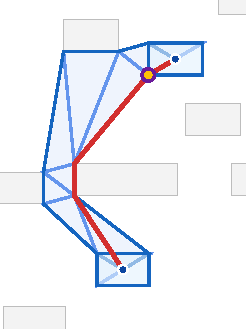
\includegraphics[width=0.9\linewidth]{sleeve_LORAS_RENLY_uncollapsed.pdf}\\[2pt]
    {\small (a) before collapse}
  \end{minipage}\hfill
  \begin{minipage}[b]{0.48\linewidth}
    \centering
    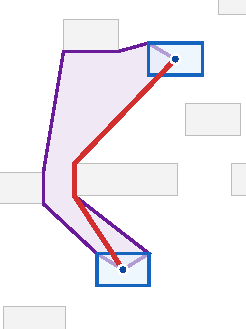
\includegraphics[width=0.9\linewidth]{sleeve_LORAS_RENLY_collapsed.pdf}\\[2pt]
    {\small (b) after collapse}
  \end{minipage}
  \caption{Effect of vertex collapse on the LORAS--RENLY edge of the Game of Thrones graph. Endpoints are shown as blue dots; their padded obstacles are highlighted in light blue. (a)~The CDT triangles forming the sleeve are drawn in cornflower blue and the funnel path in red; the thick black polyline is the perimeter of the non-collapsed sleeve. The yellow dot marks the source-obstacle vertex that gets collapsed. (b)~The sleeve after collapse, drawn as a single purple polygon with the source/target obstacles merged into the corresponding endpoints, and the funnel path (red) through it. Collapsing widens the funnel opening at the endpoint and removes the spurious detour around the obstacle corner.}
  \label{fig:collapse}
\end{figure}

%% ═══════════════════════════════════════════════════════════════════
\section{Rendering with deck.gl}
\label{sec:rendering}

The output of the build pipeline of Section~\ref{sec:tiling} is
consumed in the browser by the \texttt{TileLayer} of
\texttt{@deck.gl/geo-layers}~\cite{deckglTileLayer}. \texttt{TileLayer}
is the standard component used by online tile-map renderers: it
tracks the viewport, determines which tiles are needed at the current
zoom, and asynchronously requests them through a user-supplied
\texttt{getTileData} callback, caching the results across frames so
that subsequent pans within the cache avoid tile-data retrieval,
although visibility selection and rendering still run.

\msagljs{} integrates with this component at construction time by
exposing the precomputed pyramid as the \texttt{TileLayer}'s zoom
range, with the coarsest pyramid level mapped to the layer's lowest
zoom and the finest level to the highest. As the user pans and zooms,
\texttt{TileLayer} resolves the viewport to an integer zoom and a set
of axis-aligned tile indices and, for each tile it needs to display,
calls \texttt{getTileData}. The renderer translates each such request
back into a tile of the corresponding pyramid level and returns its
precomputed nodes, edge clips, edge labels, and arrowheads. The
mapping is one-to-one, so no rerouting or tile subdivision is performed at view
time: panning shifts the visible window over the tile cache, and
zooming selects tiles from the corresponding level. The renderer uses
\texttt{TileLayer}'s \texttt{no-overlap} refinement strategy, not an
animated cross-fade between levels.

The rendered geometry depends only on the zoom level and does not
change with the viewport, except for the clipping to the visible
window. Within each level, the displayed nodes are the ones chosen
for that level by the construction of Section~\ref{sec:filter}, and
the displayed edges use the sleeve routes and bundled edge clips
computed for those nodes, subject to the geometric limitations
described in Sections~\ref{sec:tile-build} and~\ref{sec:collapse}.

\paragraph{Interaction.}
The renderer supports pan, zoom, and hover highlighting of nodes and
edges. Hovering an edge highlights it and its incident nodes; hovering
a node highlights the node, its one-hop neighbors, and its two-hop
neighbors, each in a different color. A \texttt{zoomTo} API animates
the viewport to a target rectangle with a smooth transition and is
used, for example, by the search box to focus the view on a query
result.
%% ═══════════════════════════════════════════════════════════════════
\section{Experimental Results}
\label{sec:experiments}

We evaluate the sleeve router and the tile-pyramid build on the same benchmark graphs as Table~\ref{tab:max-per-tile}: the Game of Thrones social network~\cite{beveridge2018game}, the GD~2011 contest \texttt{composers} graph~\cite{composers}, four SNAP collaboration networks (\texttt{ca-GrQc}, \texttt{ca-HepTh}, \texttt{ca-HepPh}, \texttt{ca-CondMat}) and the SNAP \texttt{facebook\_combined} ego network~\cite{leskovec2007graph,fb}, the \texttt{deezer\_europe} social network~\cite{feather}, and the SuiteSparse Delaunay mesh \texttt{delaunay\_n15}. The loading experiments run in Chrome~153, and the routing-mode experiments in Chrome~148, on an Apple~M4~Max laptop with 48\,GB of unified memory, with the unmodified browser bundle of \msagljs{} loaded into the page. The benchmarks lay out the graphs with Pivot MDS, and the loading benchmark builds the tile pyramid with the same parameters as Table~\ref{tab:max-per-tile}: capacity~$\mathcal{C}=500$, with $Z$ chosen by the natural stops of Section~\ref{sec:tiling}.

Table~\ref{tab:perf} reports per-graph timings of three pipeline stages: \emph{Routing}, the sum of the two phases logged by the sleeve router on the full graph---constrained Delaunay triangulation of the obstacles and the Dijkstra-tree search on the CDT dual, Section~\ref{sec:sleeve}; \emph{Tiling}, the build of the tile pyramid, Section~\ref{sec:tiling}, which includes the per-level routing; and \emph{Total}, the end-to-end loading time including parsing.

\begin{table}[t]
  \caption{End-to-end loading benchmarks in Chrome~153 on an
    Apple~M4~Max laptop, all times in seconds. Measurements come from
    the \texttt{chrome-routing-bench} example, which runs the
    unmodified browser bundle of \msagljs{}. \emph{Routing} sums the
    CDT-construction and Dijkstra-tree sleeve-search phases of
    Section~\ref{sec:sleeve} on the full graph; \emph{Tiling} is the
    build of the tile pyramid, capacity $\mathcal{C}=500$ with $Z$
    chosen by the natural stops of Section~\ref{sec:tiling}, which
    includes the per-level routing; \emph{Total} is the total
    loading time including parsing of the graph file, graph layout,
    and all other stages.}
  \label{tab:perf}
  \centering
  \scriptsize
  \setlength{\tabcolsep}{6pt}
  \begin{tabular}{@{}lrrrrr@{}}
    \toprule
    Graph & $|V|$ & $|E|$ & Routing & Tiling & Total \\
    \midrule
    gameofthrones      &     407 &   2\,639 &   0.07 &   0.05 &   0.38 \\
    composers          &  3\,405 &  13\,832 &   1.63 &   0.70 &   2.85 \\
    ca-GrQc            &  5\,242 &  28\,968 &   1.85 &   0.81 &   3.43 \\
    facebook\_combined &  4\,039 &  88\,234 &   4.51 &   2.12 &   7.75 \\
    ca-HepTh           &  9\,877 &  51\,946 &   9.77 &   3.14 &  15.22 \\
    ca-HepPh           & 12\,008 & 236\,978 &  36.84 &  12.74 &  54.67 \\
    ca-CondMat         & 23\,133 & 186\,878 &  80.36 &  19.84 & 112.43 \\
    deezer\_europe     & 28\,281 &  92\,752 & 129.62 &  23.19 & 169.28 \\
    delaunay\_n15      & 32\,768 &  98\,274 &  15.93 &   5.20 &  40.02 \\
    \bottomrule
  \end{tabular}
\end{table}

CDT construction takes about 5\,ms on Game of Thrones and at most
408\,ms in this benchmark. It accounts for about $7\,\%$ of
\emph{Routing} on Game of Thrones and at most $6.3\,\%$ on the other
graphs. The remaining time is spent in the routing pass, which
includes sleeve search and path extraction, with the vertex-cover
heuristic of Section~\ref{sec:sleeve} reducing the number of trees.
The full pipeline finishes in under three minutes on all nine
graphs; this is a one-time cost for a fixed layout. The resulting
tile pyramid already contains the per-level routes, so panning and
zooming fetch and render precomputed tiles without rerouting.

Table~\ref{tab:routing-modes} isolates the contribution of the two
source-side optimizations of Section~\ref{sec:sleeve}: batched
Dijkstra trees over per-edge A* and the vertex-cover heuristic on top
of that.  Each row times a single sleeve-search pass run after layout,
with the constrained Delaunay triangulation excluded so that only the
search costs are compared. The batched Dijkstra trees outperform
per-edge A* on every social graph tested, reducing elapsed time
by up to $63$\,\% on \texttt{facebook\_combined}
and $48$\,\% on \texttt{ca-HepPh}; the vertex-cover heuristic yields
a further $11$--$42$\,\% reduction across the social graphs.
On the Delaunay mesh \texttt{delaunay\_n15}, batching alone is
$18$\,\% slower than A*. Vertex-cover reorientation recovers
$7$\,\% relative to batching alone, but remains about $10$\,\%
slower than A*. Low degree and limited shared search regions are
plausible explanations, not separately measured causes.

\begin{table}[t]
  \caption{Sleeve-search times of the three routing modes on the
    benchmark graphs of Table~\ref{tab:perf}, in
    Chrome~148. Columns: \emph{Srcs}, the number of distinct source
    endpoints in the original edge orientation, used to group DJ
    queries (A* still searches per edge); \emph{VC}, the number of
    source groups after the greedy maximum-degree vertex-cover
    reorientation of Section~\ref{sec:sleeve}; \emph{A*}, wall-clock
    seconds of one full sleeve-search pass with per-edge A*\
    (straight-line distance to the target as heuristic);
    \emph{DJ}, wall-clock seconds with the batched Dijkstra-tree
    mode---one tree per source, expanding until all of that source's
    targets are reached; \emph{VC\_DJ}, wall-clock seconds with the
    vertex-cover-reoriented Dijkstra-tree mode---same as DJ but with
    only \emph{VC}~roots (groups resolved entirely by straight-line
    tests need no tree); \emph{DJ red.}~$=$~$(\text{A*}-\text{DJ})/\text{A*}$,
    relative time reduction of DJ over A*; \emph{VC red.}~$=$~$(\text{DJ}-\text{VC\_DJ})/\text{DJ}$,
    additional time reduction of VC\_DJ over DJ. The CDT-construction phase,
    identical across modes, is excluded so that only the search costs
    are compared.}
  \label{tab:routing-modes}
  \centering
  \scriptsize
  \setlength{\tabcolsep}{1.8pt}
  \begin{tabular}{@{}lrrrrrrr@{}}
    \toprule
    & & & \multicolumn{3}{c}{Time (s)} & \multicolumn{2}{c}{Time reduction} \\
    \cmidrule(lr){4-6}\cmidrule(l){7-8}
    Graph & Srcs & VC & A* & DJ & VC\_DJ & DJ red. & VC red. \\
    \midrule
    gameofthrones      &     331 &     198 &   0.077 &   0.059 &   0.043 & $+23$\,\% & $+28$\,\% \\
    composers          &  2\,645 &  1\,281 &   2.60  &   2.14  &   1.49  & $+18$\,\% & $+31$\,\% \\
    ca-GrQc            &  5\,241 &  2\,796 &   2.55  &   2.52  &   1.65  &  $+1$\,\% & $+35$\,\% \\
    facebook\_combined &  3\,663 &  3\,045 &  13.31  &   4.88  &   4.36  & $+63$\,\% & $+11$\,\% \\
    ca-HepTh           &  9\,875 &  5\,003 &  17.13  &  15.42  &   9.28  & $+10$\,\% & $+40$\,\% \\
    ca-HepPh           & 12\,006 &  7\,032 & 111.2   &  58.07  &  36.38  & $+48$\,\% & $+37$\,\% \\
    ca-CondMat         & 23\,133 & 13\,564 & 189.1   & 131.1   &  76.45  & $+31$\,\% & $+42$\,\% \\
    deezer\_europe     & 21\,060 & 13\,450 & 172.1   & 154.0   & 124.4   & $+11$\,\% & $+19$\,\% \\
    delaunay\_n15      & 28\,467 & 23\,456 &  13.57  &  16.02  &  14.88  & $-18$\,\% &  $+7$\,\% \\
    \bottomrule
  \end{tabular}
\end{table}

\paragraph{Browsing smoothness.}
We test how smoothly a user can browse a freshly loaded graph in the
browser. On the same M4~Max laptop as Tables~\ref{tab:perf} and
\ref{tab:routing-modes}, a script loads a graph, waits for the tile
pyramid to build, and then runs two trials of three dives each
(six dives per graph). Each dive picks
a random point inside the laid-out graph, recenters the view on that
point, zooms from the coarsest view all the way in to the finest
detail in one second, then zooms back out to the coarsest view in
another second. The three dives in each trial run back to back.
These browsing runs use separately built pyramids; their recorded
level counts are reported in Table~\ref{tab:smoothness} and differ
from the natural-stop builds in Table~\ref{tab:max-per-tile}.
The two tables should therefore not be read as measurements of
identical tile pyramids.

While the dives play, the script measures three things on the
browser side. First, the interval between successive animation-frame
callbacks, whose nominal spacing at $60$\,Hz is $16.7$\,ms. We report
the arithmetic mean of the two trial-specific $95$th percentiles,
not a pooled percentile or a direct measurement of displayed frames.
Second, the number and total duration of main-thread tasks lasting
more than $50$\,ms, summed over both trials. Such ``long tasks'' can
delay rendering and input handling. Third, at
the deepest point of every dive, how many graphical objects the
browser must draw, that is, nodes, edge clips, labels, and
arrowheads, summed over visible tiles intersecting the viewport.
We report the maximum of these six samples. This count is a proxy
for rendering load, not a GPU-time measurement or a maximum over
all frames. Table~\ref{tab:smoothness} reports the result.

\begin{table}[t]
  \caption{Browsing-smoothness measurements on the benchmark graphs.
    For each graph the script runs two trials of three dives; each dive picks
    a random point inside the laid-out graph, recenters on it, and
    zooms from the coarsest view to the finest and back in two
    seconds. \emph{Levels}, number of tile-pyramid levels built
    ($Z+1$);
    \emph{LT}, number of main-thread tasks longer than $50$\,ms
    summed over both trials; \emph{LT total}, their total
    duration, in milliseconds; \emph{Frame p95}, the
    mean of the two trial-specific $95$th percentiles of
    animation-frame callback intervals, in milliseconds;
    \emph{Elts max}, the largest number of graphical objects,
    that is, nodes, edge clips, labels, and arrowheads, that the
    browser had to draw at the deepest point of any dive.}
  \label{tab:smoothness}
  \centering
  \scriptsize
  \setlength{\tabcolsep}{2pt}
  \begin{tabular}{@{}lrrrrrrr@{}}
    \toprule
    Graph & $|V|$ & $|E|$ & Levels & LT & \shortstack{LT\\total} & \shortstack{Frame\\p95} & \shortstack{Elts\\max} \\
    \midrule
    gameofthrones      &     407 &   2\,639 & 5 &  0 &     0 &  17.4 &   2\,567 \\
    composers          &  3\,405 &  13\,832 & 9 &  1 &    51 &  18.2 &      497 \\
    ca-GrQc            &  5\,242 &  28\,968 & 9 &  0 &     0 &  18.2 &      677 \\
    ca-HepTh           &  9\,877 &  51\,946 & 9 &  0 &     0 &  18.2 &      383 \\
    facebook\_combined &  4\,039 &  88\,234 & 9 &  0 &     0 &  18.0 &      495 \\
    ca-HepPh           & 12\,008 & 236\,978 & 9 &  9 &   556 &  18.4 &   1\,394 \\
    ca-CondMat         & 23\,133 & 186\,878 & 9 &  5 &   273 &  18.2 &   1\,391 \\
    deezer\_europe     & 28\,281 &  92\,752 & 9 &  3 &   164 &  18.4 &   2\,505 \\
    delaunay\_n15      & 32\,768 &  98\,274 & 9 &  0 &     0 &  18.1 &   1\,012 \\
    \bottomrule
  \end{tabular}
\end{table}

The mean trial-specific frame-interval percentiles are
$17.4$--$18.4$\,ms after rounding, close to the nominal
$16.7$\,ms interval at $60$\,Hz. These statistics do not rule out
longer stalls or establish perceptual smoothness. There are nine,
five, and three long tasks on \texttt{ca-HepPh},
\texttt{ca-CondMat}, and \texttt{deezer\_europe}, respectively,
one on \texttt{composers}, and none on the remaining graphs.
At the sampled deepest zooms, the browser is asked to draw at most
$2\,567$ objects on \texttt{gameofthrones} and at most $2\,505$ on
\texttt{deezer\_europe} even though the latter graph has $35$ times
more edges. This is the property the pyramid is designed to deliver:
the draw workload is tied to visible tile contents rather than
requiring the full graph to be drawn each frame. This is an
empirical observation, not a graph-size-independent complexity bound.

\paragraph{Evaluation scope.}
The loading and routing-mode tables report individual runs, not
repeated-run means with confidence intervals. The browsing experiment
covers only six sampled locations per graph on one machine, and
some samples contain no graph entities. It does not establish
worst-case frame times, performance on lower-end hardware, or user
task effectiveness. We also lack a controlled comparison with
non-tiled rendering and a quantitative measure of visual stability
across level changes.

%% ═══════════════════════════════════════════════════════════════════
\section{Conclusion}
\label{sec:conclusion}

We presented \msagljs{}, an open-source TypeScript library for graph layout, edge routing, and visualization in web browsers. The sleeve routing method routes edges directly on the CDT dual graph using batched Dijkstra trees and the funnel algorithm. The tiling scheme enables map-like exploration of large graphs with level-of-detail filtering and edge simplification. The WebGL renderer, built on deck.gl, provides smooth pan-and-zoom interaction.

\paragraph{Future work.} The current approach builds the entire tile
pyramid up front, which is expensive and bounds the size of graphs we
can handle. A natural next step is to build only the first few levels
quickly and hand them to the renderer; the remaining levels would be
built lazily as the user browses the graph. This
could lower the time-to-first-frame and reduce resident tile storage,
but layout, routing, and graph storage would still limit graph size.

A second challenge is that some tiles can contain many more
elements than the capacity parameter~$\mathcal{C}$ that guides the
build. Table~\ref{tab:max-per-tile} reports densest tiles holding
approximately 5.8$\times$ the nominal $\mathcal{C}$ in the worst cases, which leaves
the rendering and interaction cost uneven across the viewport.
Enforcing an actual per-tile budget remains an open problem.

%% ═══════════════════════════════════════════════════════════════════
\section*{Supplemental Materials}
\label{sec:supplemental_materials}
\msagljs{} is available
\ifthenelse{\boolean{gdanonymous}}{as open source; an anonymized
mirror of the repository is provided for review at
\url{\anonsource}}{as open source at \url{\canonsource} and as the
NPM packages \texttt{@msagl/core}, \texttt{@msagl/drawing},
\texttt{@msagl/parser}, \texttt{@msagl/renderer-svg}, and
\texttt{@msagl/renderer-webgl}, all on \url{https://www.npmjs.com/}}.
A live demo of the WebGL renderer with sleeve routing is available at
\anondemourl{\anondemowebgl}{https://microsoft.github.io/msagljs/renderer-webgl-sleeve/index.html}.
The benchmark drivers used for
Tables~\ref{tab:max-per-tile}--\ref{tab:smoothness} ship with the
repository.

\acknowledgments{%
Generative AI was used throughout the preparation of this article and
the accompanying software, including writing and refactoring source
code, generating figures, drafting and editing technical prose, and
running tests and benchmarks. The authors reviewed all AI-assisted
content and take responsibility for the final form.}

\bibliographystyle{abbrv-doi}
\bibliography{main}

\end{document}
